% !TEX program = xelatex
\documentclass[10pt,letterpaper,twocolumn]{article}

% === GEOMETRY ===
\usepackage[top=0.75in, bottom=0.75in, left=0.75in, right=0.75in]{geometry}

% === FONTS ===
\usepackage{fontspec}
\usepackage{unicode-math}

\setmainfont{Latin Modern Roman}
\setsansfont{Latin Modern Sans}

% Custom AC fonts
\newfontfamily\acbold{ywft-processing-bold}[
  Path=../../system/public/type/webfonts/,
  Extension=.ttf
]
\newfontfamily\aclight{ywft-processing-light}[
  Path=../../system/public/type/webfonts/,
  Extension=.ttf
]
\newfontfamily\kidlispfont{ComicRelief-Regular}[
  Path=../arxiv-kidlisp/fonts/,
  Extension=.ttf
]
\newfontfamily\kidlispbold{ComicRelief-Bold}[
  Path=../arxiv-kidlisp/fonts/,
  Extension=.ttf
]
\setmonofont{Latin Modern Mono}[Scale=0.85]

% === PACKAGES ===
\usepackage{xcolor}
\usepackage{titlesec}
\usepackage{enumitem}
\usepackage{booktabs}
\usepackage{tabularx}
\usepackage{fancyhdr}
\usepackage{hyperref}
\usepackage{graphicx}
\graphicspath{{figures/}{../arxiv-kidlisp/figures/}}
\usepackage{ragged2e}
\usepackage{microtype}
\usepackage{listings}
\usepackage{natbib}
\usepackage[colorspec=0.92]{draftwatermark}

% === COLORS (AC palette) ===
\definecolor{acpink}{RGB}{180,72,135}
\definecolor{acpurple}{RGB}{120,80,180}
\definecolor{acdark}{RGB}{64,56,74}
\definecolor{acgray}{RGB}{119,119,119}
\definecolor{klbrand}{RGB}{205,92,155}
\definecolor{klcyan}{RGB}{112,214,255}
\definecolor{kldark}{RGB}{48,43,58}
\definecolor{draftcolor}{RGB}{205,92,155}

% === DRAFT WATERMARK ===
\DraftwatermarkOptions{
  text=ARBEJDSUDKAST,
  fontsize=3cm,
  color=draftcolor!18,
  angle=45,
  pos={0.5\paperwidth, 0.5\paperheight}
}

% === KIDLISP SYNTAX COLORS ===
\definecolor{klfn}{RGB}{0,136,170}
\definecolor{klform}{RGB}{119,51,170}
\definecolor{klrepeat}{RGB}{170,0,170}
\definecolor{klnum}{RGB}{204,0,102}
\definecolor{klstr}{RGB}{170,120,0}
\definecolor{klcmt}{RGB}{102,102,102}
\definecolor{klmath}{RGB}{0,136,0}
\definecolor{klvar}{RGB}{204,102,0}
\definecolor{klembed}{RGB}{0,136,0}

% KidLisp inline color macros
\newcommand{\kn}[1]{\textcolor{klnum}{#1}}
\newcommand{\kt}[1]{\textcolor{klstr}{#1}}
\newcommand{\kv}[1]{\textcolor{klvar}{#1}}
\newcommand{\ke}[1]{\textcolor{klembed}{\textbf{#1}}}
\newcommand{\km}[1]{\textcolor{klmath}{#1}}

% === HYPERREF ===
\hypersetup{
  colorlinks=true,
  linkcolor=acpurple,
  urlcolor=acpurple,
  citecolor=acpurple,
  pdfauthor={@jeffrey},
  pdftitle={KidLisp-kort: Programmer der kan v\ae re p\aa\ et kort},
}

% === SECTION FORMATTING ===
\titleformat{\section}
  {\normalfont\bfseries\normalsize\uppercase}
  {\thesection.}
  {0.5em}
  {}
\titlespacing{\section}{0pt}{1.2em}{0.3em}

\titleformat{\subsection}
  {\normalfont\bfseries\small}
  {\thesubsection}
  {0.5em}
  {}
\titlespacing{\subsection}{0pt}{0.8em}{0.2em}

% === HEADER/FOOTER ===
\pagestyle{fancy}
\fancyhf{}
\renewcommand{\headrulewidth}{0pt}
\fancyhead[C]{\footnotesize\color{acpink}\textit{Arbejdsudkast --- ikke til citation}}
\fancyfoot[C]{\footnotesize\thepage}

% === CUSTOM COMMANDS ===
\newcommand{\acdot}{{\color{acpink}.}}
\newcommand{\kidlisp}{\textsc{KidLisp}}

% === LISTINGS ===
\lstdefinelanguage{kidlisp}{
  morekeywords=[1]{wipe,ink,line,box,circle,tri,plot,flood,shape,zoom,scroll,spin,blur,contrast,embed,layer,width,height,frame,time,wiggle,melody,mic,suck,sort,form,trans,cube,move,scale,hop,overtone,resolution,write,text,type,stamp,paste,point,poly,noise,fade,pan,unpan,mask,unmask,flip,crawl,left,right,up,down,goto,face,outline,fill,stroke},
  morekeywords=[2]{def,let,if,cond,once,later,lambda,do},
  morekeywords=[3]{repeat},
  morekeywords=[4]{random,sin,cos,tan,floor,ceil,round,abs,sqrt,min,max},
  sensitive=true,
  morecomment=[l]{;},
  morestring=[b]",
  escapeinside={|}{|},
}
\lstset{
  language=kidlisp,
  basicstyle=\ttfamily\small,
  keywordstyle=[1]\color{klfn}\bfseries,
  keywordstyle=[2]\color{klform}\bfseries,
  keywordstyle=[3]\color{klrepeat}\bfseries,
  keywordstyle=[4]\color{klmath},
  commentstyle=\color{klcmt}\itshape,
  stringstyle=\color{klstr},
  breaklines=true,
  frame=single,
  rulecolor=\color{acgray!30},
  backgroundcolor=\color{acgray!5},
  xleftmargin=0.5em,
  xrightmargin=0.5em,
  aboveskip=0.5em,
  belowskip=0.5em,
}

\lstdefinelanguage{python}{
  morekeywords={def,return,import,from,class,if,else,for,in,with,as,try,except,None,True,False,self,and,or,not,lambda,yield,pass,break,continue,raise,while},
  sensitive=true,
  morecomment=[l]{\#},
  morestring=[b]",
  morestring=[b]',
}
\lstset{
  language=kidlisp,
}

% === LIST SETTINGS ===
\setlist[itemize]{nosep, leftmargin=1.2em, itemsep=0.1em}
\setlist[enumerate]{nosep, leftmargin=1.2em}

% === COLUMN SEPARATION ===
\setlength{\columnsep}{1.8em}

% === PARAGRAPH SETTINGS ===
\setlength{\parindent}{1em}
\setlength{\parskip}{0.3em}

\tolerance=800
\emergencystretch=1em
\hyphenpenalty=50

\begin{document}

% ============ TITLE BLOCK ============

\twocolumn[{%
\begin{center}

\includegraphics[height=4em]{pals}\par\vspace{0.5em}
{\kidlispbold\fontsize{24pt}{28pt}\selectfont\color{kldark} Kid{\color{klbrand}Lisp}-kort}\par
\vspace{0.2em}
{\kidlispfont\fontsize{11pt}{13pt}\selectfont\color{klbrand} Programmer der kan v\ae re p\aa\ et kort}\par
\vspace{0.6em}
{\normalsize\href{https://prompt.ac/@jeffrey}{@jeffrey}}\par
{\small\color{acgray} Aesthetic\acdot Computer}\par
{\small\color{acgray} ORCID: \href{https://orcid.org/0009-0007-4460-4913}{0009-0007-4460-4913}}\par
\vspace{0.3em}
{\small\color{acpurple} \url{https://kidlisp.com} \enspace$\cdot$\enspace \url{https://aesthetic.computer}}\par
\vspace{0.6em}
\rule{\textwidth}{1.5pt}
\vspace{0.5em}
\end{center}

\begin{center}
{\small\color{acpink}\textbf{[ arbejdsudkast --- ikke til citation ]}}
\end{center}
\vspace{0.3em}

\begin{quote}
\small\noindent\textbf{Abstrakt.}
\kidlisp{}-programmer er korte. Et typisk program best\aa r af 2--4 linjer S-udtryk, der producerer en komplet visuel komposition---en stjerneburst, en spiral, et t\ae ppe, en fraktal. Denne korthed er ikke tilf\ae ldig men designet: sproget udelader brugerdefinerede funktioner, rekursion og abstraktionsmekanismer, s\aa\ programmer forbliver flade og l\ae sbare. Vi observerer, at denne fladhed skaber en naturlig korrespondance mellem programmer og fysiske kort. Et \kidlisp{}-program, dets kildekode og dets renderede output kan sameksistere p\aa\ et enkelt trykt kort. Denne artikel beskriver \emph{KidLisp Cards}-formatet---et s\ae t programmer organiseret efter visuel kategori---og en Python-renderingspipeline (PIL-baseret fortolker), der producerer kortbilleder uden for browseren. Vi diskuterer, hvad kort er nu (en kurateret notesbog af visuelle koaner), hvad de kunne blive (byttekort, p\ae dagogiske sekvenser, trykte partiturer, postkunst), og hvordan kortbegr\ae nsningen p\aa virker sprogdesignet.
\end{quote}
\vspace{0.5em}
}]

% ============ 1. INTRODUKTION ============

\section{Introduktion}

De fleste programmeringssprog producerer programmer, der er for lange til at trykke p\aa\ et kartotekskort. Dette er en konsekvens af abstraktion: generelle programmeringssprog opmuntrer til nedbrydning i funktioner, klasser, moduler og filer. Programmet er fordelt over en kodebase. Ingen enkelt artefakt fanger helheden.

\kidlisp{} er anderledes. Dets programmer er typisk 1--6 linjer lange. En komplet animeret scene, et geometrisk m\o nster, en rekursiv fraktal eller et moir\'{e}-interferensm\o nster kan v\ae re i f\aa\ S-udtryk. Dette er ikke en begr\ae nsning men et designvalg: \kidlisp{} udelader brugerdefinerede funktioner, rekursion (undtagen gennem \texttt{later}), mutable datastrukturer og imports. Programmer er flade sekvenser af tegnekommandoer, l\o kker og betingelser.

Denne fladhed skaber en mulighed. Hvis kildekoden til et program kan v\ae re p\aa\ et kort, og det visuelle output af det program kan v\ae re p\aa\ det samme kort, s\aa\ bliver kortet en selvst\ae ndig artefakt: et program du kan holde, give til nogen, s\ae tte p\aa\ en v\ae g eller sende med posten. Kortet er b\aa de dokumentation og eksekverbart. Det er et \emph{partitur}---instruktioner til at producere en visuel begivenhed.

Denne artikel beskriver KidLisp Cards-formatet (\S\ref{sec:format}), offline-renderingspipelinen (\S\ref{sec:pipeline}), det aktuelle kortkatalog (\S\ref{sec:catalog}), layoutvariationer og deres sociale og fysiske affordanser (\S\ref{sec:layouts}) samt spekulative fremtider for formatet (\S\ref{sec:futures}).

% ============ 2. KORTFORMATET ============

\section{Kortformatet}
\label{sec:format}

Et KidLisp-kort har tre elementer:

\begin{enumerate}
  \item \textbf{Titel.} Et kort navn der fremkalder det visuelle output: ``Starburst,'' ``Honeycomb,'' ``Spiral Walk.''
  \item \textbf{Renderet output.} Et pixel-art-billede (160$\times$120 standardopl\o sning, opskaleret 3$\times$ med nearest-neighbor-interpolation for at bevare skarpe kanter).
  \item \textbf{Kildekode.} Det komplette \kidlisp{}-program, typisk 1--4 linjer, vist i monospace under billedet.
\end{enumerate}

Kortet er selvst\ae ndigt: enhver der l\ae ser kildekoden kan reproducere billedet pr\ae cist, i enhver \kidlisp{}-fortolker. Der er ingen eksterne afh\ae ngigheder, ingen imports, ingen konfiguration. Programmet \emph{er} kortet.

\subsection{Kortdimensioner}

Det renderede billede fylder et 160$\times$120 pixel-l\ae rred (4:3-format), svarende til standard \kidlisp{}-opl\o sningen. Ved 3$\times$ opskalering producerer dette et 480$\times$360 pixel-billede egnet til sk\ae rmvisning. Til tryk er kort dimensioneret som 4$\times$6 tommer (standard kartotekskort / postkort), med billedet i den \o vre del og kildekoden nedenunder.

\subsection{Hvad g\o r et godt kort}

Ikke ethvert \kidlisp{}-program giver et godt kort. De bedste kort deler egenskaber:

\begin{itemize}
  \item \textbf{Korthed.} 1--4 linjer. Hvis kildekoden ikke passer komfortabelt under billedet, er programmet for langt til formatet.
  \item \textbf{Overraskelse.} Outputtet b\o r v\ae re mere komplekst eller smukt end kildekoden antyder. Et tre-linjers program der producerer et moir\'{e}-m\o nster belønner n\ae rmere inspektion.
  \item \textbf{L\ae sbarhed.} En l\ae ser b\o r kunne f\o lge fra kilde til output uden at k\o re programmet. Forbindelsen mellem kode og billede b\o r v\ae re synlig, selv om den ikke er umiddelbart indlysende.
  \item \textbf{Uafh\ae ngighed.} Ingen \texttt{\$code}-indlejringer, ingen ekstern tilstand. Kortet skal fungere isoleret.
\end{itemize}

\begin{figure}[t]
\centering
\fbox{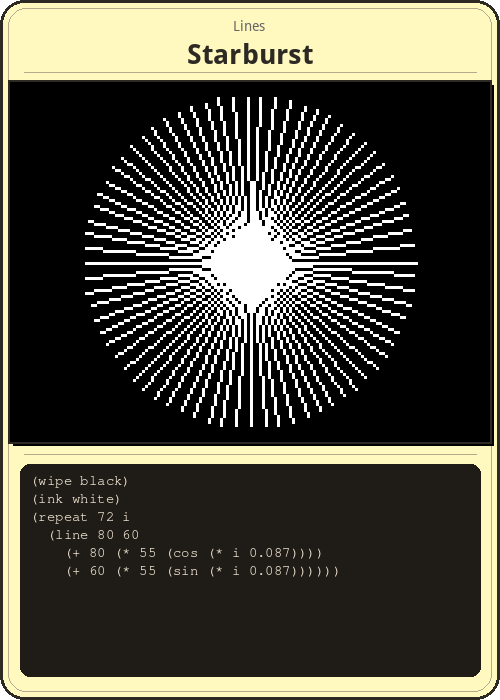
\includegraphics[width=0.47\columnwidth]{card-starburst.png}}%
\hfill%
\fbox{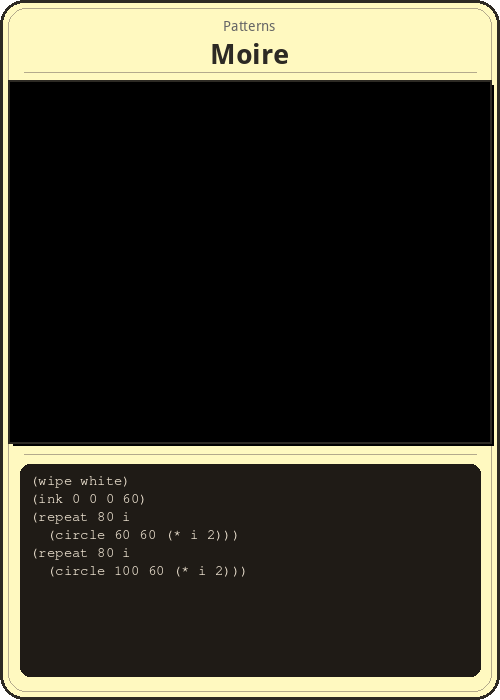
\includegraphics[width=0.47\columnwidth]{card-moire.png}}
\caption{To programkort renderet af Python-fortolkeren: ``Starburst'' (72 radiale linjer, 3 linjer kode) og ``Moir\'{e}'' (overlappende koncentriske cirkler, 3 linjer). Disse er trivielle eksempler---de demonstrerer kortformatets struktur men repr\ae senterer ikke sprogets udtryksevne eller formatets ambitioner.}
\label{fig:program-cards}
\end{figure}

% ============ 3. RENDERINGSPIPELINE ============

\section{Offline-renderingspipeline}
\label{sec:pipeline}

KidLisp-kort renderes med en Python-fortolker der k\o rer uden for browseren. Dette muligg\o r batch-rendering, trykproduktion og notesbog-baseret kuratering uden at kr\ae ve den fulde Aesthetic\acdot Computer-runtime.

\subsection{Python-fortolkeren}

Fortolkeren (\texttt{notebooks/ac.py}, 452 linjer) implementerer en delm\ae ngde af \kidlisp{} tilstr\ae kkelig til statisk kortrendering:

\begin{itemize}
  \item \textbf{Tegning:} \texttt{wipe}, \texttt{ink}, \texttt{line}, \texttt{box}, \texttt{circle}, \texttt{tri}, \texttt{plot}, \texttt{shape}, \texttt{flood}
  \item \textbf{Skildpadde:} \texttt{crawl}, \texttt{left}, \texttt{right}, \texttt{goto}, \texttt{face}, \texttt{up}, \texttt{down}
  \item \textbf{Kontrol:} \texttt{repeat}, \texttt{if}, \texttt{def}, \texttt{later}, \texttt{do}
  \item \textbf{Matematik:} fuld aritmetik, trigonometri, \texttt{abs}, \texttt{sqrt}, \texttt{min}, \texttt{max}
  \item \textbf{L\ae rred:} \texttt{resolution}, \texttt{fill}, \texttt{outline}, \texttt{stroke}
\end{itemize}

Fortolkeren bruger PIL (Pillow) til rendering. Hvert kort tegnes p\aa\ et RGBA-l\ae rred, opskaleres med nearest-neighbor-interpolation og eksporteres som PNG. Python-implementeringen er bevidst simplere end browser-evaluatoren (15.161 linjer)---den udelader animation, lyd, indlejring og timing-syntaks og fokuserer udelukkende p\aa\ den delm\ae ngde der er n\o dvendig for statisk visuelt output.

\subsection{Jupyter Notebook-arbejdsgang}

Det prim\ae re kurateringsv\ae rkt\o j er en Jupyter-notesbog (\texttt{notebooks/kidlisp-cards.ipynb}). Funktionen \texttt{show\_card()} renderer et program og viser det inline som et HTML-kort:

\begin{lstlisting}[language=python,basicstyle=\ttfamily\footnotesize]
show_card("Starburst", """(wipe black)
(ink white)
(repeat 72 i
  (line 80 60
    (+ 80 (* 55 (cos (* i 0.087))))
    (+ 60 (* 55 (sin (* i 0.087))))))""")
\end{lstlisting}

Hvert kald producerer et kort med m\o rk baggrund med titel, renderet billede og kildekode vist inline. Notesbogen fungerer b\aa de som udviklingsmilj\o\ og galleri---at scrolle gennem notesbogen er som at bladre i et s\ae t kort.

\subsection{To fortolkere, \'{e}t sprog}

Eksistensen af to uafh\ae ngige fortolkere (JavaScript i browseren, Python i notesbogen) tjener som en krydsvalideringsmekanisme. Hvis et program renderes identisk i begge, er dets adf\ae rd bestemt udelukkende af sprogets semantik snarere end implementeringsdetaljer. Programmer der afh\ae nger af browserspecifikke funktioner (animation, lyd, indlejrede lag) udelukkes fra kortformatet pr. konstruktion---de renderer simpelthen ikke i Python-fortolkeren.

% ============ 4. KORTKATALOG ============

\section{Kortkataloget}
\label{sec:catalog}

Den aktuelle notesbog indeholder 28 kort organiseret i syv kategorier. Hver kategori udforsker et andet aspekt af sproget gennem minimale eksempler. Disse programmer er bevidst trivielle---tegne\o velser, matematiske illustrationer, skildpaddeg\aa ture. De etablerer kortformatets struktur men repr\ae senterer ikke dets udtryksm\ae ssige potentiale. De interessante kort er endnu ikke lavet. Formatets v\ae rdi vil fremkomme fra programmer der bruger korthed til at sige noget v\ae rd at sige, ikke fra geometriske demoer.

\subsection{Linjer}

Linjekort demonstrerer \texttt{repeat} og trigonometri. En stjerneburst udsender 72 linjer fra centrum. En krydsarkering overlejrer vandrette og lodrette gitre med lav opacitet.

\begin{figure}[h]
\centering
\fbox{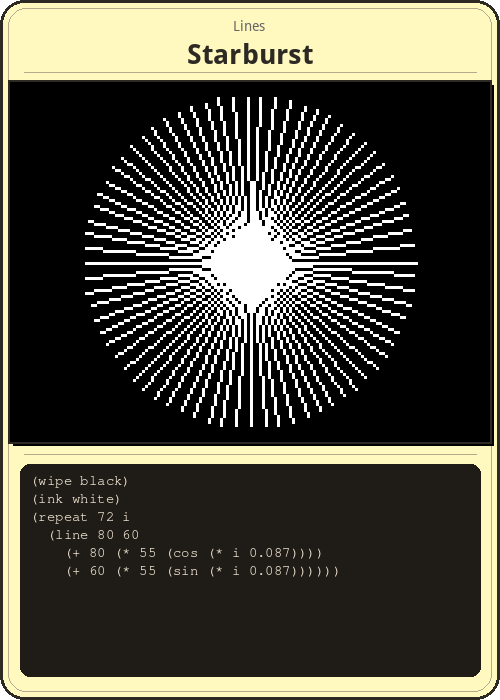
\includegraphics[width=0.47\columnwidth]{card-starburst.png}}%
\hfill%
\fbox{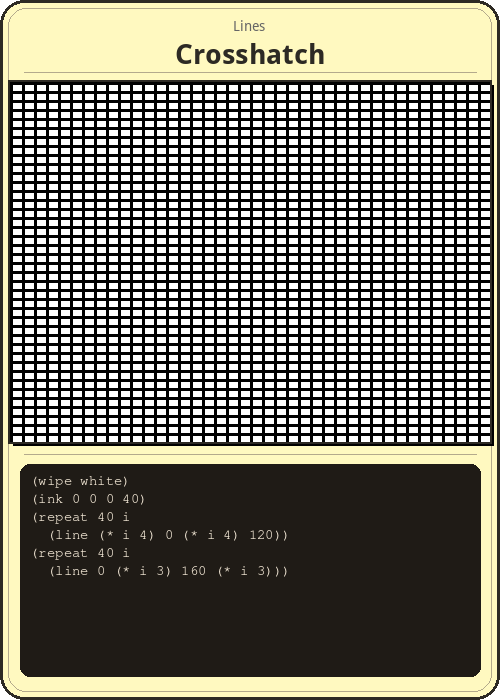
\includegraphics[width=0.47\columnwidth]{card-crosshatch.png}}
\caption{``Starburst'' og ``Crosshatch'' --- linjekort.}
\label{fig:lines}
\end{figure}

\begin{lstlisting}
; Starburst — 72 radial lines
(wipe |\kt{black}|)
(ink |\kt{white}|)
(repeat |\kn{72}| |\kv{i}|
  (line |\kn{80}| |\kn{60}|
    (|\km{+}| |\kn{80}| (|\km{*}| |\kn{55}| (|\km{cos}| (|\km{*}| |\kv{i}| |\kn{0.087}|))))
    (|\km{+}| |\kn{60}| (|\km{*}| |\kn{55}| (|\km{sin}| (|\km{*}| |\kv{i}| |\kn{0.087}|))))))
\end{lstlisting}

\subsection{Cirkler}

Cirkelkort bruger \texttt{outline}-tilstand og indlejrede \texttt{repeat}-l\o kker. ``Ripple'' tegner 30 koncentriske cirkler med bl\aa skiftende farve.

\begin{figure}[h]
\centering
\fbox{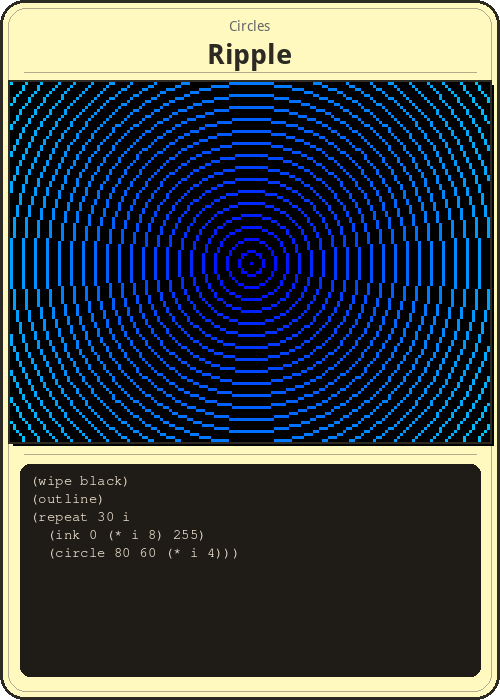
\includegraphics[width=0.47\columnwidth]{card-ripple.png}}%
\hfill%
\fbox{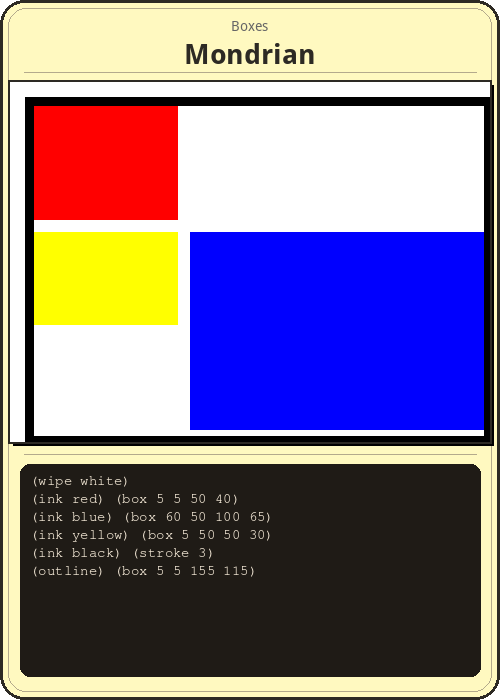
\includegraphics[width=0.47\columnwidth]{card-mondrian.png}}
\caption{``Ripple'' (cirkler) og ``Mondrian'' (bokse).}
\label{fig:circles-boxes}
\end{figure}

\subsection{Bokse \& komposition}

``Mondrian'' genskaber det prim\ae rfarvede gitter med fire farvede rektangler. ``Nest'' tegner 10 indrykkede rektangler med skiftende nuancer.

\subsection{Matematik \& kurver}

Disse kort bruger \texttt{plot} med matematiske funktioner. ``Lissajous'' tegner en Lissajous-figur med 600 punkter. ``Spiral'' plotter en pol\ae r spiral.

\begin{figure}[h]
\centering
\fbox{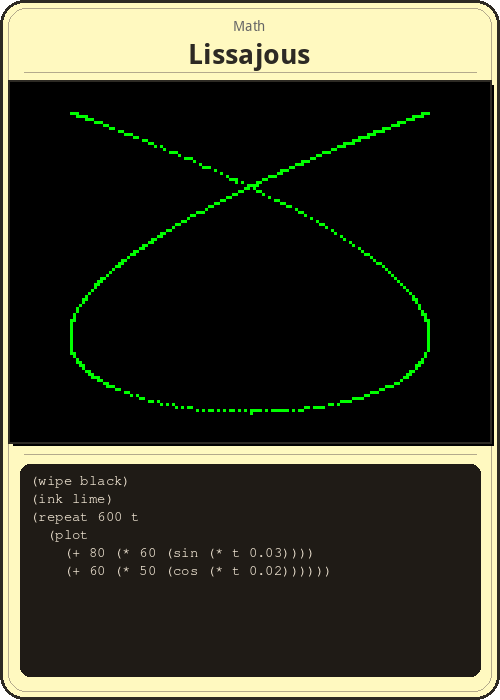
\includegraphics[width=0.47\columnwidth]{card-lissajous.png}}%
\hfill%
\fbox{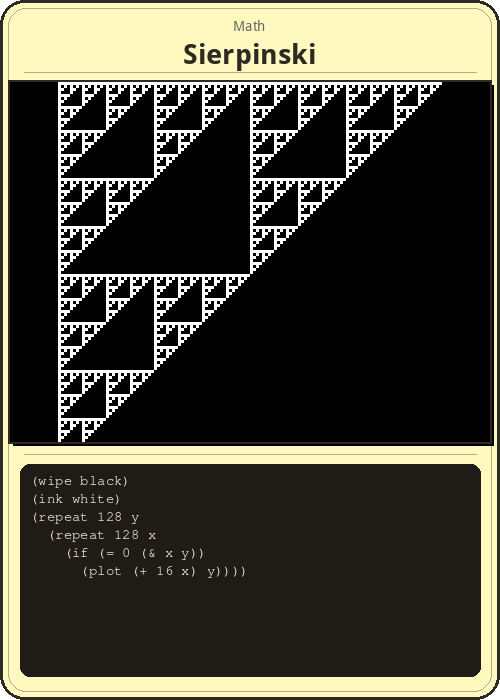
\includegraphics[width=0.47\columnwidth]{card-sierpinski.png}}
\caption{``Lissajous'' (matematiske kurver) og ``Sierpinski'' (bitwise AND-fraktal).}
\label{fig:math}
\end{figure}

\subsection{Farve \& gradienter}

``Sierpinski'' bruger bitwise AND til at generere Sierpinski-trekanten: \texttt{(if (= 0 (\& x y)) (plot (+ 16 x) y))}. ``Sunflower'' plotter 500 punkter langs en gylden-vinkel-spiral med cykliske farver.

\subsection{Skildpaddegrafik}

Skildpaddekort bruger \texttt{crawl}, \texttt{left}, \texttt{right} og \texttt{face}. En femtakket stjerne bruger \texttt{(right 144)}. Et tr\ae\ bruger \texttt{later} til rekursiv forgrening. En snefnug indlejrer Koch-kurvesegmenter.

\begin{figure}[h]
\centering
\fbox{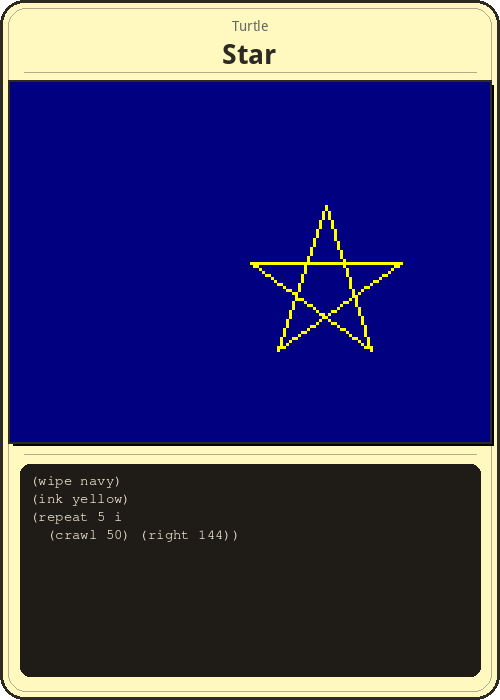
\includegraphics[width=0.47\columnwidth]{card-star.png}}%
\hfill%
\fbox{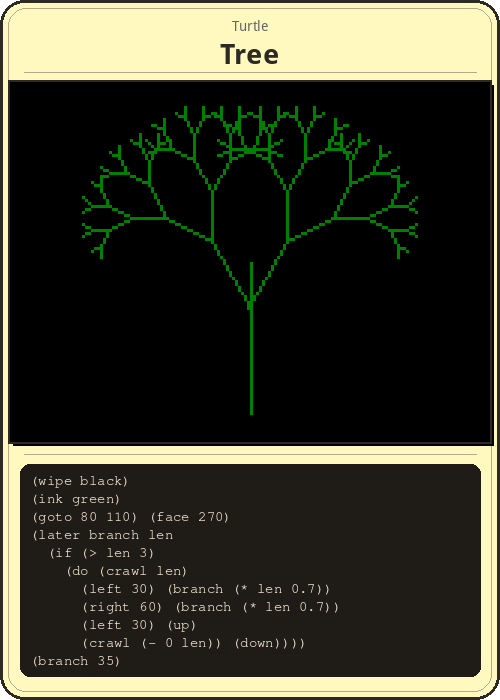
\includegraphics[width=0.47\columnwidth]{card-tree.png}}
\caption{``Star'' og ``Tree'' --- skildpaddegrafikkort.}
\label{fig:turtle}
\end{figure}

\begin{lstlisting}
; Star — 5 sides, 144-degree turns
(wipe |\kt{navy}|)
(ink |\kt{yellow}|)
(repeat |\kn{5}| |\kv{i}| (crawl |\kn{50}|) (right |\kn{144}|))
\end{lstlisting}

\subsection{Minimale koaner}

De korteste kort i s\ae ttet. ``Horizon'' er tre linjer: m\o rk himmel, gylden jord. ``Pip'' er en enkelt r\o d prik p\aa\ sort. Disse kort n\ae rmer sig det minimale levedygtige program---den mindste m\ae ngde kode der producerer et genkendeligt billede.

\begin{figure}[h]
\centering
\fbox{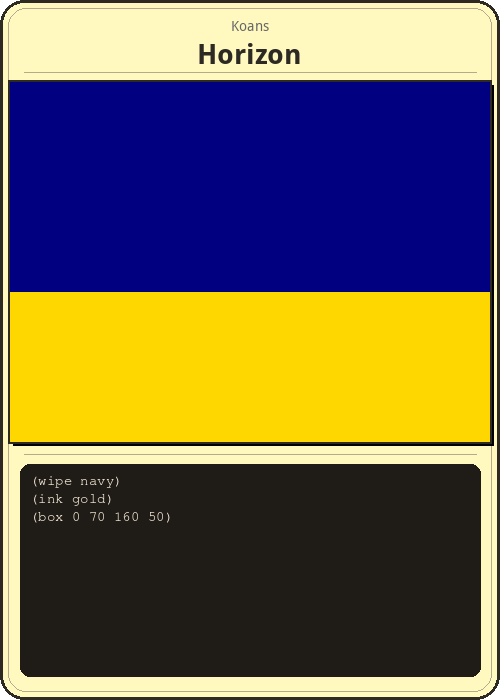
\includegraphics[width=0.47\columnwidth]{card-horizon.png}}%
\hfill%
\fbox{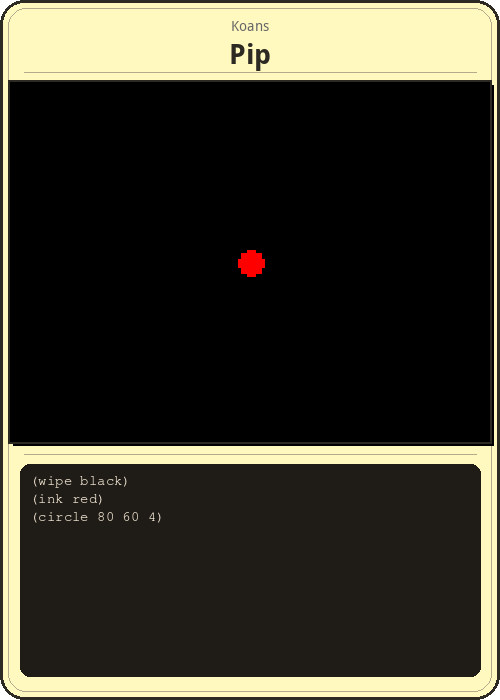
\includegraphics[width=0.47\columnwidth]{card-pip.png}}
\caption{``Horizon'' og ``Pip'' --- minimale koaner (2--3 linjer hver).}
\label{fig:koans}
\end{figure}

\begin{lstlisting}
; Pip — the minimum card
(wipe |\kt{black}|)
(ink |\kt{red}|)
(circle |\kn{80}| |\kn{60}| |\kn{4}|)
\end{lstlisting}

\begin{figure*}[t]
\centering
\fbox{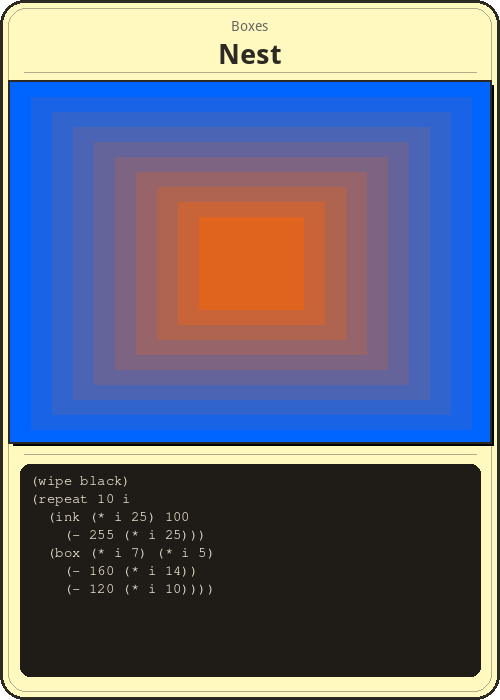
\includegraphics[height=5.5cm]{card-nest.png}}%
\hfill%
\fbox{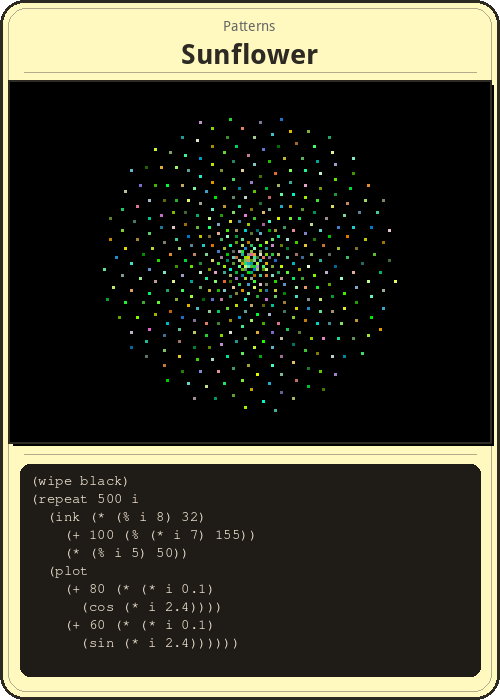
\includegraphics[height=5.5cm]{card-sunflower.png}}%
\hfill%
\fbox{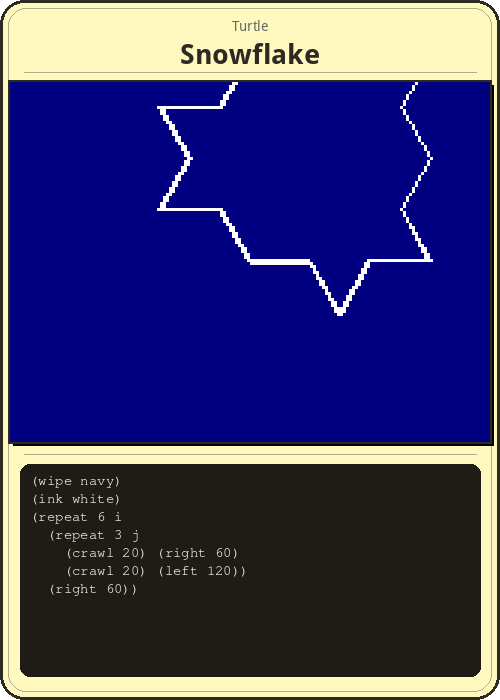
\includegraphics[height=5.5cm]{card-snowflake.png}}%
\hfill%
\fbox{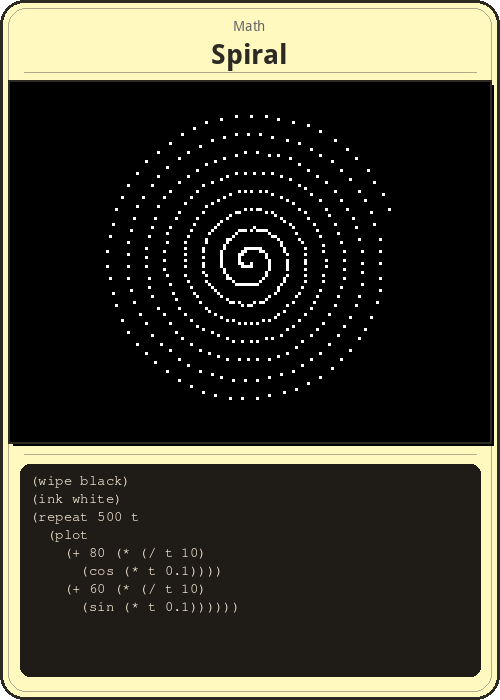
\includegraphics[height=5.5cm]{card-spiral.png}}
\caption{Fire komplette kort der viser formatet: titel, renderet output og kildekode. Fra venstre mod h\o jre: ``Nest,'' ``Sunflower,'' ``Snowflake,'' ``Spiral.'' Hvert kort er selvst\ae ndigt---kildekoden under billedet er det komplette program. Disse er trivielle tegne\o velser, ikke udtryk for formatets potentiale.}
\label{fig:four-cards}
\end{figure*}

% ============ 5. LAYOUTS ============

\section{Layouts}
\label{sec:layouts}

Kortformatet har intet fast layout. Hvordan de tre elementer (titel, output, kilde) arrangeres bestemmer hvad kortet afforderer---hvad du kan g\o re med det fysisk og socialt. Dette afsnit udforsker layoutvariationer og deres konsekvenser.

\begin{figure*}[t]
\centering
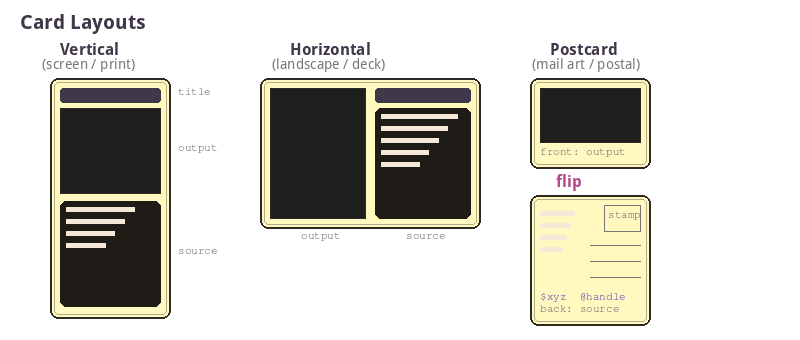
\includegraphics[width=\textwidth]{layout-comparison.png}
\caption{Tre layoutstrategier. \textbf{Vertikal:} titel / billede / kilde stablet fra top til bund, optimeret til telefonsk\ae rme og portr\ae ttryk. \textbf{Horisontal:} billede til venstre, titel og kilde til h\o jre, velegnet til landskabskort og side-om-side-gennemsyn. \textbf{Postkort:} renderet output p\aa\ forsiden, kildekode og metadata p\aa\ bagsiden---et kort der kan sendes med posten, hvor programmet er skjult indtil man vender det.}
\label{fig:layouts}
\end{figure*}

\subsection{Vertikal (sk\ae rm / tryk)}

Standardlayoutet stabler titel, billede og kilde fra top til bund. Dette er notesbog-layoutet---det scroller naturligt p\aa\ en telefon eller i en Jupyter-notesbog. Til tryk passer det til et 4$\times$6 tommers kort i portr\ae tformat. L\ae serens \o je bev\ae ger sig nedad fra navn til billede til kode og f\o lger forholdet mellem programmet og dets output.

\subsection{Horisontal (s\ae t / landskab)}

Et landskabslayout placerer det renderede billede til venstre og kildekoden til h\o jre. Dette fungerer til at sprede kort ud over et bord, til pr\ae sentationer og til sammenligning side om side. To kort placeret ved siden af hinanden skaber et diptyk---betragteren kan sammenligne programmer og output samtidigt.

\subsection{Postkort (postkunst)}

Postkortlayoutet adskiller forside fra bagside. Forsiden viser kun det renderede billede, fuld udblødning, ingen tekst. Bagsiden viser kildekoden, forfatterens handle, kortkoden (\texttt{\$xyz}) og et frim\ae rkeomr\aa de. Modtageren ser billedet f\o rst---en visuel artefakt. At vende kortet afsl\o rer programmet: instruktionerne der producerede det. Kortet er b\aa de kunstobjekt og eksekverbart partitur, afh\ae ngigt af hvilken side man l\ae ser.

\begin{figure*}[h]
\centering
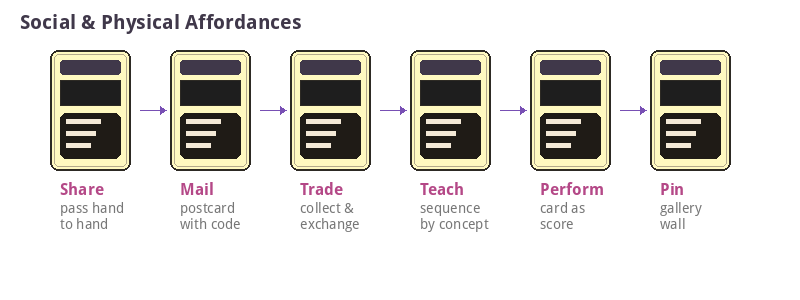
\includegraphics[width=\textwidth]{layout-affordances.png}
\caption{Sociale og fysiske affordanser ved kortformatet. Hver affordans f\o lger af kortets materialitet: det kan \textbf{deles} fra h\aa nd til h\aa nd, \textbf{sendes} som postkort, \textbf{byttes} og samles, \textbf{undervises} fra i p\ae dagogiske sekvenser, \textbf{opf\o res} som et grafisk partitur eller \textbf{s\ae ttes op} p\aa\ en galleriv\ae g.}
\label{fig:affordances}
\end{figure*}

\subsection{S\ae tarrangementer}

Kort er ikke enkeltobjekter. De danner s\ae t, og arrangementet af et s\ae t skaber mening. En \emph{p\ae dagogisk sekvens} ordner kort efter koncept: bokse f\o rst (koordinater), derefter linjer (trigonometri), derefter cirkler (radius og gentagelse), derefter matematiske kurver (plot og sinus), derefter skildpaddegrafik (relativ bev\ae gelse) og til sidst koaner (minimalt udtryk). Et \emph{gallerigitter} arrangerer kort rumligt p\aa\ en v\ae g og inviterer til sammenligning p\aa\ tv\ae rs af kategorier. Et \emph{blandet s\ae t} randomiserer r\ae kkef\o lgen og producerer uventede sammenstillinger mellem en fraktal og en horisont, mellem et tr\ae\ og en prik.

\begin{figure}[h]
\centering
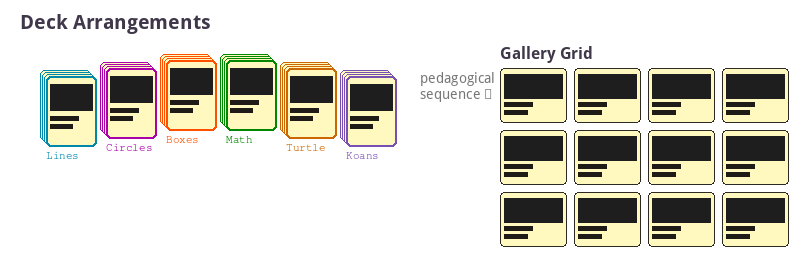
\includegraphics[width=\columnwidth]{layout-decks.png}
\caption{S\ae tarrangementer. Venstre: kort spredt ud efter kategori (linjer, cirkler, bokse, matematik, skildpadde, koaner) med flere kort stablet per kategori. H\o jre: et gallerigitter hvor kort er arrangeret rumligt til gennemsyn.}
\label{fig:decks}
\end{figure}

% ============ 6. KORT I DEN VIRKELIGE VERDEN ============

\section{Kort i den virkelige verden}
\label{sec:wild}

Notesbogskortene er \o velser. Det egentlige \kidlisp{}-korpus---16.000+ programmer skabt af 59 forfattere---indeholder v\ae rker der bruger den fulde runtime: animation, lyd, indlejrede lag, gradientfading, tilf\ae ldig placering og timing-syntaks. Disse v\ae rker er korte nok til kortformatet men langt mere udtryksfulde end notesbog-eksemplerne. Deres forh\aa ndsvisningsbilleder renderes af oven-tjenesten (Puppeteer-baseret sk\ae rmoptagelse) og serveres via CDN.

\begin{figure*}[t]
\centering
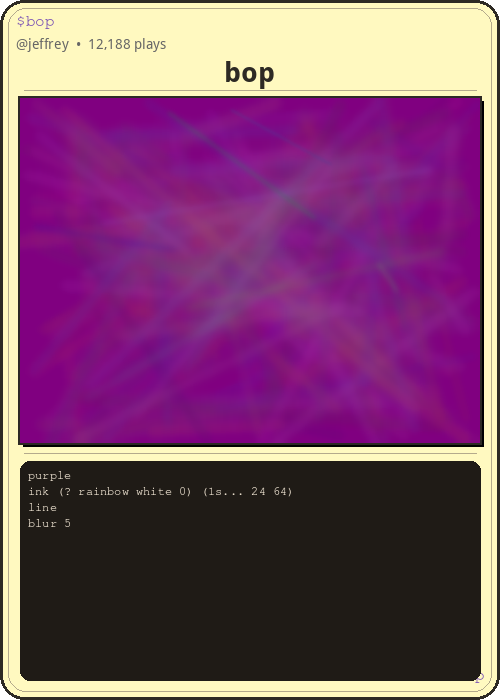
\includegraphics[height=7cm]{user-card-bop.png}%
\hfill%
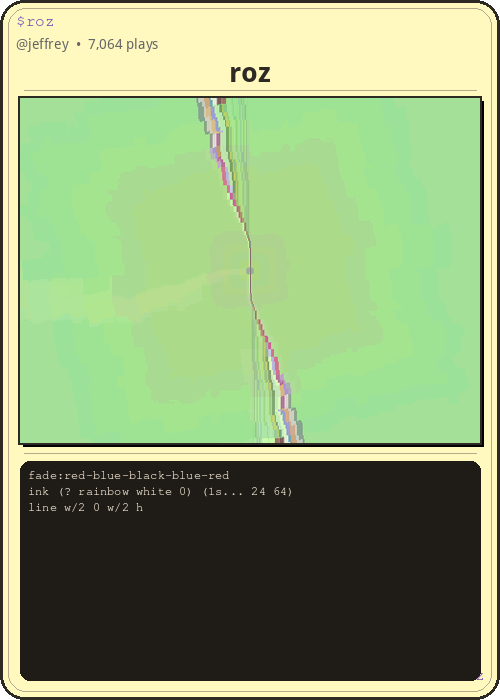
\includegraphics[height=7cm]{user-card-roz.png}%
\hfill%
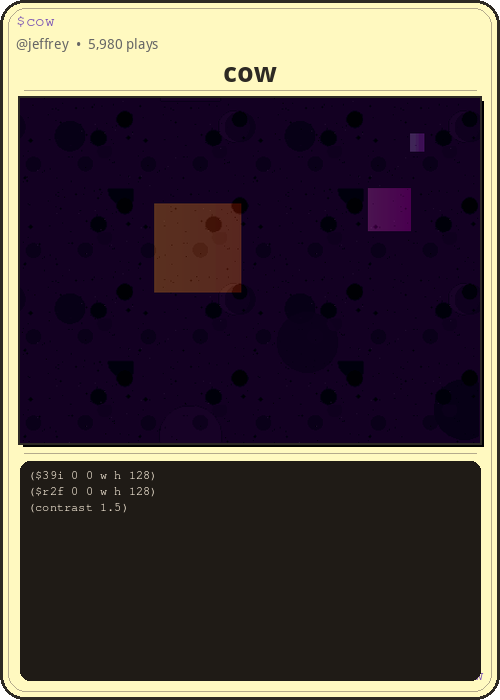
\includegraphics[height=7cm]{user-card-cow.png}%
\hfill%
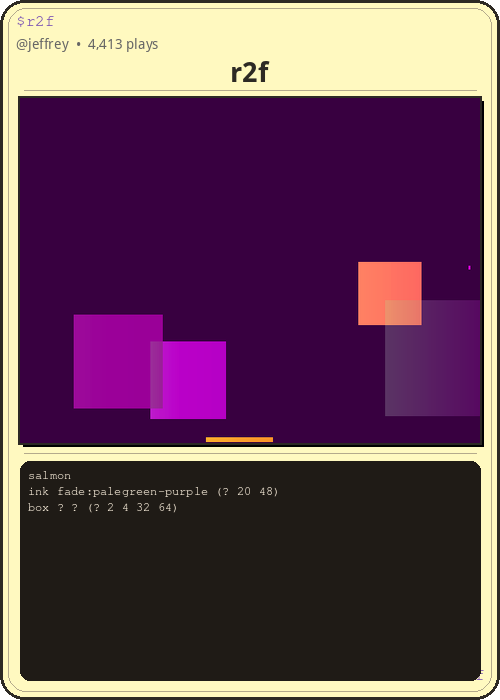
\includegraphics[height=7cm]{user-card-r2f.png}
\caption{Fire kort fra det levende \kidlisp{}-korpus, renderet af oven-tjenesten. Fra venstre mod h\o jre: \texttt{\$bop} (12.188 afspilninger---det mest popul\ae re v\ae rk, 4 linjer), \texttt{\$roz} (7.064 afspilninger, 3 linjer), \texttt{\$cow} (5.980 afspilninger---en komposition der indlejrer to andre v\ae rker via \texttt{\$39i} og \texttt{\$r2f}), \texttt{\$r2f} (4.413 afspilninger, 3 linjer med tilf\ae ldig boksplacering). Alle af @jeffrey. Disse programmer bruger funktioner der ikke findes i Python-fortolkeren---animation, tilf\ae ldighed (\texttt{?}), gradientfading (\texttt{fade:}), indlejrede lag (\texttt{\$code})---men deres kildekode passer stadig p\aa\ et kort.}
\label{fig:user-cards}
\end{figure*}

\subsection{Hvad rigtige v\ae rker tilf\o jer}

Notesbogskortene bruger en statisk delm\ae ngde af \kidlisp{}. Rigtige v\ae rker p\aa\ \texttt{kidlisp.com} bruger den fulde runtime:

\begin{itemize}
  \item \textbf{Animation.} Programmer re-evalueres hvert frame. \texttt{frame} og \texttt{time} \ae ndres automatisk. Et enkelt-frame-sk\ae rmbillede fanger \'{e}t \o jeblik af et levende v\ae rk.
  \item \textbf{Tilf\ae ldighed.} \texttt{?}-operatoren producerer en tilf\ae ldig v\ae rdi fra en liste hvert frame. \texttt{(ink (? red blue green))} flimrer mellem farver.
  \item \textbf{Gradientfading.} \texttt{fade:red-blue-black} interpolerer en fler-stops-gradient over l\ae rredet, drevet af \texttt{frame}-t\ae llingen. \'{E}t udtryk erstatter sider af manuel farvematematik.
  \item \textbf{Indlejring.} \texttt{(\$cow)} henter v\ae rket \texttt{cow} fra MongoDB, evaluerer det i en offscreen-buffer og sammens\ae tter resultatet. V\ae rker bygger p\aa\ v\ae rker.
  \item \textbf{Timing.} \texttt{1s... (zoom 0.5)} anvender en zoom hvert sekund. Ingen eksplicit animationsl\o kke.
\end{itemize}

Disse funktioner holder programmer korte mens de dramatisk udvider hvad de kan udtrykke. \texttt{\$bop}---det mest afspillede v\ae rk med 12.188 visninger---er fire linjer: en lilla baggrund, regnbueflikrende bl\ae k, en tilf\ae ldig linje og en sl\o ring. P\aa\ et kort ligner det et frosset \o jeblik af et kinetisk maleri. I browseren er det \'{e}t.

\subsection{Kortet som \o jebliksbillede}

Et kort af et animeret v\ae rk er n\o dvendigvis ufuldst\ae ndigt. Det fanger \'{e}t frame af en temporal proces. Denne ufuldst\ae ndighed er en del af formatet: kortet inviterer dig til at taste koden og se hvad den rent faktisk g\o r. Det statiske billede er et l\o fte. Kildekoden er opfyldelsen. Kortkoden (\texttt{\$bop}) er broen---tast den ind p\aa\ \texttt{kidlisp.com} og kortet kommer til live.

% ============ 7. HVAD KORT KUNNE BLIVE ============

\section{Hvad kort kunne blive}
\label{sec:futures}

Kortformatet er ungt. Den aktuelle notesbog er et proof of concept---28 programmer renderet offline. Men korrespondancen mellem korte programmer og fysiske kort antyder flere retninger.

\subsection{Byttekort}

Et KidLisp-kort er samlev\ae rdigt p\aa\ en m\aa de som det meste software ikke er. Hvert kort har et navn, en visuel identitet, en kortkode (\texttt{\$xyz}) og en forfatter. Kort kunne trykkes, nummereres og byttes. Sj\ae ldne kort kunne bruge obskure sprogfunktioner eller producere uventet komplekst output fra minimal kode. ``Sj\ae ldenheden'' af et kort er dets informationst\ae thed: hvor meget visuel kompleksitet der opst\aa r fra hvor f\aa\ tegn.

\subsection{P\ae dagogiske sekvenser}

De syv kategorier i den aktuelle notesbog antyder en undervisningsr\ae kkef\o lge: start med bokse (simple koordinater), g\aa\ videre til linjer (trigonometri), cirkler (radius og gentagelse), matematiske kurver (plot og sinus), skildpaddegrafik (relativ bev\ae gelse) og til sidst koaner (minimalt udtryk). Hvert kort underviser i \'{e}t koncept. En l\ae rer kunne give elever et fysisk s\ae t og bede dem reproducere hvert kort, modificere det eller skabe et nyt kort i samme kategori.

\subsection{Trykte partiturer}

I musik er et partitur instruktioner til at producere en temporal begivenhed. Et KidLisp-kort er instruktioner til at producere en visuel begivenhed. Kort kunne fungere som grafiske partiturer i traditionen fra Cornelius Cardew, John Cage og Fluxus-begivenhedspartiturer. En opf\o rer modtager et kort, fortolker koden (ved at taste den ind p\aa\ \texttt{kidlisp.com}, ved at l\ae se den h\o jt, ved at tegne den i h\aa nden) og producerer en begivenhed. Kortet er partituret. Renderingen er \'{e}n mulig realisering.

\subsection{Postkunst}

Ved 4$\times$6 tommer er et KidLisp-kort et postkort. Forsiden viser det renderede billede. Bagsiden viser kildekoden, forfatterens handle og kortkoden til at sl\aa\ det op online. Postkunst med eksekverbart indhold---modtageren kan taste koden og se billedet genskabt p\aa\ deres sk\ae rm. Det fysiske kort og det digitale program er det samme v\ae rk i to medier.

\subsection{Generativt papirvarer}

Fordi Python-fortolkeren er deterministisk og selvst\ae ndig, kan kort batch-renderes til trykproduktion uden netv\ae rksadgang. Et s\ae t kort kunne trykkes som et h\ae fte, et zine eller et s\ae t i \ae ske. Pipelinen \texttt{cards-convert.mjs} producerer allerede 4$\times$6 tommers PDF-kort fra papirformatet; at udvide dette til at inkludere renderet programoutput sammen med kildekode er et naturligt n\ae ste skridt.

\subsection{Begr\ae nsning som generativt princip}

Den mest interessante konsekvens af kortformatet er hvordan det p\aa virker sproget. Programmer der ikke passer p\aa\ et kort antyder manglende abstraktioner---eller antyder at programmet g\o r for meget. Kortbegr\ae nsningen opmuntrer til \o konomi: find tre-linjers-programmet der producerer det mest interessante billede. Dette er en generativ begr\ae nsning i Oulipo-traditionen---vilk\aa rlige formelle restriktioner der producerer uventede kreative resultater.

% ============ 6. RELATERET ARBEJDE ============

\section{Relateret arbejde}

\textbf{Trykt kode.} Demoscene-traditionen med ``sizecoding'' (programmer under 256 bytes) deler \ae stetikken med minimale programmer der producerer maksimalt output. \kidlisp{}-kort er t\ae ttere p\aa\ ``kodedigt''-traditionen, hvor selve kildekoden l\ae ses som tekst sammen med dens output.

\textbf{Grafiske partiturer.} Cardews \emph{Treatise} (1967) og Cages \emph{Notations} (1969) etablerede at visuel notation kan tjene som opf\o relsesinstruktioner uden at foreskrive en specifik realisering. KidLisp-kort adskiller sig ved at de er fuldt eksekverbare---renderingen er deterministisk, ikke \aa ben for fortolkning. Men kort-som-partitur-indramningen inviterer til genfortolkning: hvad nu hvis man ``spiller'' kortet anderledes hver gang?

\textbf{Byttekortspil.} Spil som \emph{Magic: The Gathering} (1993) demonstrerede at kort med strukturerede metadata (navn, type, regeltekst, kunst) skaber rige kombinatoriske rum. KidLisp-kort har naturlige metadata (titel, kategori, funktionsantal, linjeantal, output-kompleksitet) der kunne underst\o tte lignende spilmekanikker.

\textbf{Beregningsmæssige notesbøger.} Jupyter-notesbøger kombinerer allerede kode og output. KidLisp Cards-notesbogen er en Jupyter-notesbog, men med en specifik begr\ae nsning: hver celle er et selvst\ae ndigt kort snarere end et trin i en l\ae ngere beregning. Notesbogen er et galleri, ikke en fort\ae lling.

% ============ 7. KONKLUSION ============

\section{Konklusion}

KidLisp-kort udspringer af en simpel observation: n\aa r programmer er korte nok, passer de p\aa\ kort. Kortformatet---titel, billede, kilde---g\o r programmer til fysiske artefakter der kan trykkes, sendes med posten, samles, undervises fra og opf\o res. Python-renderingspipelinen muligg\o r offline batchproduktion. Kataloget med syv kategorier giver et kurateret indgangspunkt til sproget.

Formatet er et igangv\ae rende arbejde. Det aktuelle s\ae t p\aa\ 28 kort er et udgangspunkt, ikke en f\ae rdig samling. Sp\o rgsm\aa let er ikke hvor mange kort der skal laves, men hvilke programmer der fortjener at v\ae re kort---hvilke tre-linjers kompositioner der producerer billeder v\ae rd at holde i h\aa nden.

Notesbogen, fortolkeren og kortkataloget er tilg\ae ngelige p\aa\ \url{https://github.com/whistlegraph/aesthetic-computer}. Programmer kan oprettes og deles p\aa\ \url{https://kidlisp.com}.

\vspace{0.5em}
\noindent\textbf{ORCID:} \href{https://orcid.org/0009-0007-4460-4913}{0009-0007-4460-4913}

% ============ REFERENCER ============

\bibliographystyle{plainnat}
\bibliography{references}

\end{document}
